%yright 2007, 2008, 2009 Elsevier Ltd
%% 
%% This file is part of the 'Elsarticle Bundle'.
%% ---------------------------------------------
%% 
%% It may be distributed under the conditions of the LaTeX Project Public
%% License, either version 1.2 of this license or (at your option) any
%% later version.  The latest version of this license is in
%%    http://www.latex-project.org/lppl.txt
%% and version 1.2 or later is part of all distributions of LaTeX
%% version 1999/12/01 or later.
%% 
%% The list of all files belonging to the 'Elsarticle Bundle' is
%% given in the file `manifest.txt'.
%% 

%% Template article for Elsevier's document class `elsarticle'
%% with numbered style bibliographic references
%% SP 2008/03/01

% \documentclass[preprint,11pt]{elsarticle}
\documentclass[final,1p,11pt]{elsarticle}

%\documentclass[final,1p,times]{elsarticle}


%% Use the option review to obtain double line spacing
%%\documentclass[authoryear,preprint,review,12pt]{elsarticle}

%% Use the options 1p,twocolumn; 3p; 3p,twocolumn; 5p; or 5p,twocolumn
%% for a journal layout:
%% \documentclass[final,1p,times]{elsarticle}
%% \documentclass[final,1p,times,twocolumn]{elsarticle}
%% \documentclass[final,3p,times]{elsarticle}
%% \documentclass[final,3p,times,twocolumn]{elsarticle}
%% \documentclass[final,5p,times]{elsarticle}
%% \documentclass[final,5p,times,twocolumn]{elsarticle}

%%% For including figures, graphicx.sty has been loaded in
%% elsarticle.cls. If you prefer to use the old commands
%% please give \usepackage{epsfig}


\usepackage{epsfig}
%\usepackage{cite}
%\usepackage{mcite}
\usepackage{array,tabularx,epsfig,mathrsfs,graphicx,rotating}
\usepackage{ifthen}
\usepackage{amsfonts}
\usepackage{ragged2e}
\PassOptionsToPackage{hyphens}{url}
\usepackage[hyphens]{url}
\usepackage{hyperref}
\usepackage{listings}
\usepackage{lineno}
\usepackage{subfigure}
\usepackage{epstopdf}
% Custom colors
\usepackage{color}
\usepackage{float}
\usepackage{verbatim}
\usepackage{color,soul}

% to cross text
\usepackage[normalem]{ulem} % either use this (simple) or
\usepackage{soul} % use this (many fancier options)
\usepackage{amsmath,amssymb}

\let\originallesssim\lesssim
\let\originalgtrsim\gtrsim

\DeclareRobustCommand{\lesssim}{%
  \mathrel{\mathpalette\lowersim\originallesssim}%
}
\DeclareRobustCommand{\gtrsim}{%
  \mathrel{\mathpalette\lowersim\originalgtrsim}%
}

\makeatletter
\newcommand{\lowersim}[2]{%
  \sbox\z@{$#1<$}%
  \raisebox{-\dimexpr\height-\ht\z@}{$\m@th#1#2$}%
}
\makeatother


\hypersetup{
  colorlinks=true,
  linkcolor=blue,
  citecolor=blue,
  urlcolor=blue
}




\graphicspath{{figs/}}


\pdfinfo{
   /Author (Chekanov et al)
   /Title  (Studies of granularity of a hadronic calorimeter for tens-of-TeV jets  at a 100 TeV pp collider)
   /CreationDate (D:2017)
   /Subject (PDFLaTeX)
   /Keywords (PDF;LaTeX)
}


\textheight=22cm
\textwidth=14.5cm

\newcommand{\beq}{\begin{equation}}
\newcommand{\eeq}{\end{equation}}
\newcommand{\la}{\langle}
\newcommand{\promc}{{\sc ProMC}}
\newcommand{\ra}{\rangle}
\newcommand{\eps}{\epsilon}
\newcommand{\ud}{\mathrm{d}}
\newcommand{\Ec}{\mathcal{E}}
\newcommand{\Fc}{\mathcal{F}}
\newcommand{\Za}{\mathrm{Z_1}}
\newcommand{\Zb}{\mathrm{Z_2}}
\newcommand{\Zn}{\mathrm{Z_n}}
\newcommand{\F}{\mathrm{F}}

\chardef\til=126
\newcommand{\GEANTfour} {\textsc{geant4}}
\newcommand{\pythia} {\textsc{Pythia8~}}
\newcommand{\pt}{\ensuremath{p_{\mathrm{T}}}}


\journal{}

\begin{document}
%\hfill ANL-HEP-149528
\definecolor{mygreen}{rgb}{0,0.6,0} \definecolor{mygray}{rgb}{0.5,0.5,0.5} \definecolor{mymauve}{rgb}{0.58,0,0.82}

\lstset{ %
 backgroundcolor=\color{white},   % choose the background color; you must add \usepackage{color} or \usepackage{xcolor}
 basicstyle=\footnotesize,        % the size of the fonts that are used for the code
 breakatwhitespace=false,         % sets if automatic breaks should only happen at whitespace
 breaklines=true,                 % sets automatic line breaking
 captionpos=b,                    % sets the caption-position to bottom
 commentstyle=\color{mygreen},    % comment style
 deletekeywords={...},            % if you want to delete keywords from the given language
 escapeinside={\%*}{*)},          % if you want to add LaTeX within your code
 extendedchars=true,              % lets you use non-ASCII characters; for 8-bits encodings only, does not work with UTF-8
 keepspaces=true,                 % keeps spaces in text, useful for keeping indentation of code (possibly needs columns=flexible)
 frame=tb,
 keywordstyle=\color{blue},       % keyword style
 language=Python,                 % the language of the code
 otherkeywords={*,...},            % if you want to add more keywords to the set
 rulecolor=\color{black},         % if not set, the frame-color may be changed on line-breaks within not-black text (e.g. comments (green here))
 showspaces=false,                % show spaces everywhere adding particular underscores; it overrides 'showstringspaces'
 showstringspaces=false,          % underline spaces within strings only
 showtabs=false,                  % show tabs within strings adding particular underscores
 stepnumber=2,                    % the step between two line-numbers. If it's 1, each line will be numbered
 stringstyle=\color{mymauve},     % string literal style
 tabsize=2,                        % sets default tabsize to 2 spaces
 title=\lstname,                   % show the filename of files included with \lstinputlisting; also try caption instead of title
 numberstyle=\footnotesize,
 basicstyle=\small,
 basewidth={0.5em,0.5em}
}


\begin{frontmatter}

\title{
FCC-notes\\
Studies of the timing for tens-of-TeV jets  at a 100~TeV $pp$ collider 
}
%%%%%%%%%%%%%%%%%%%%%%%%%%%%%%%%%%%%%%%%%%%%%%%%%%%%%%%%%%%%%%%

\author[add3]{C.-H. Yeh}
\ead{a9510130375@gmail.com}

\author[add1]{S.V.~Chekanov}
\ead{chekanov@anl.gov}

\author[addDuke]{A.V.~Kotwal}
\ead{ashutosh.kotwal@duke.edu}

\author[add1]{J.~Proudfoot}
\ead{proudfoot@anl.gov}

\author[addDuke]{S.~Sen}
\ead{sourav.sen@duke.edu}

\author[add2]{N.V.~Tran}
\ead{ntran@fnal.gov}

\author[add3]{S.-S.~Yu}
\ead{syu@cern.ch}

\address[add3]{
Department of Physics and Center for High Energy and High Field Physics, 
National Central University, Chung-Li, Taoyuan City 32001, Taiwan
}

\address[add1]{
HEP Division, Argonne National Laboratory,
9700 S.~Cass Avenue,
Argonne, IL 60439, USA. 
}

\address[addDuke]{
Department of Physics, Duke University, USA
}

\address[add2]{
Fermi National Accelerator Laboratory
}




\begin{abstract}
This is the document for noting the timing resources. I've drafted some of them and tried my best to write down the detail for all of them. Until now, we have been doing the study with the truth-level data, and we will move on to the RECO-level study later.

\end{abstract}

\begin{keyword}
multi-TeV physics, $pp$ collider, future hadron colliders, FCC, SppC
\end{keyword}
\end{frontmatter}



%%%%%%%%%%%%%%%%%%%%%%%%%%%%%%%%%%%%%%%%%%%%%%%%%%%%%%%%%%%%%%%%%%
\section{Introduction}
%%%%%%%%%%%%%%%%%%%%%%%%%%%%%%%%%%%%%%%%%%%%%%%%%%%%%%%%%%%%%%%%%%

%%%%%%%%%%%%%% sections 
\section{Definitions used in the studies}
\label{sec:Def_timing}
\subsection{Timing}
At the first place, the definition of the timing should be obtained as our benchmark to be the variable of distinguishing different number of subjet(s) in a large raduis jet. The standard formula of the timing is as follows for each particle:
\begin{equation}
 Timing = \frac{L(\eta)}{V(V_{x},V_{y},V_{z})}  
\end{equation}
Basically, it is the normal formula of the time of flight(TOF), depending on the different \(\eta\), leading to the different distances\(\ L\) between collision point and HCAL barrel, along with the three-dimensional velocities\(\ V \) of the particles.\\

But, since the effect of the magnetic field is taken into account, the timing used in this paper is the modified one with only considering the Z direction of the distance and velocity, and then we can get more precise value of the timing by the truth of the Z-direction trace of the particle isn't changed by the magnetic field. The formula used in this paper is as follows: 
\begin{equation}
 Timing = \frac{L_{z}}{V(V_{z})} 
\end{equation}

After applying this formula on all particles, and the timing can be used as a great variable for distinguishing many things in the detector. 

\subsection{Trailing particle - PT and T}
The definition of the trailing particles defined by the Timing(T) and transverse momentum(PT) should be clarified as well. We have two categories of the trailing particles
\begin{enumerate}
\item Defined by the timing, we called it "trailing-T", meaning that the particle has the longest traveling timing in the jet. 
\item Defined by the PT, we called it "trailing-PT", meaning that the lowest-PT particle in the jet. 
\end{enumerate}
Consequently, we can define next-to trailing particle as well, such as the second long traveling timing-"next-to-trailing-T" or the second low PT-"next-to-trailing-PT", and so on.
%%%%%%%%%%%%%%% commented out 
\end{comment}


\section{Studies of the components of the jet ( Include pre-selection )}
\label{sec:Def_timing}

Since the events of the HCAl barrel would be used as our candidates in order to avoid mixing up with the events flying to the endcap, and also the consistent of calculating the timing as well,  \(\eta <1\) cut is used to be our first pre-selection.\\ 

Considering the effect of the magnetic field is another issue that we should recognize. Since 5T magnetic field is applied, we can figure out the minimum PT that particle should have to arrive the HCAL barrel. In the end, 1.5GeV cut is applied as our second pre-selection and you can see there are a little bit pions cut off because of their low PT.\\

Theoretically, in our cases of WW and qq fragmentation, they should have the same fraction of the different kinds of particles in their large radius jet since both of them have the quark(s) be their final state. We've done checking the fractions of the different particles in these two processes. Please look at the picture~\ref{Jet_com}.\\

According to the plots, before and after the \(\eta\)\ cut, the fractions of the different particles are the same, and after cutting off the low-PT particles, the fractions don't change much but lose few pions (Relatively, the photon goes up). It is the expected circumstance and tells us that the jets could be used in our studies.

\begin{figure}
\begin{center}
   \subfigure[5TeV] {
   \includegraphics[width=0.45\textwidth]{/Users/ms08962476/singularity/TIming_Studies/Codes/5TeV/Try_Trailing_ID_Eta_cut_no_with_withPT_5TeV.pdf}
   }
   \subfigure[10TeV] {
   \includegraphics[width=0.45\textwidth]{/Users/ms08962476/singularity/TIming_Studies/Codes/10TeV/Try_Trailing_ID_Eta_cut_no_with_withPT_10TeV.pdf}
   }
   \subfigure[20TeV] {
   \includegraphics[width=0.45\textwidth]{/Users/ms08962476/singularity/TIming_Studies/Codes/20TeV/Try_Trailing_ID_Eta_cut_no_with_withPT_20TeV.pdf}
   }
    \subfigure[40TeV] {
   \includegraphics[width=0.45\textwidth]{/Users/ms08962476/singularity/TIming_Studies/Codes/40TeV/Try_Trailing_ID_Eta_cut_no_with_withPT_40TeV.pdf}
   }
\end{center}
\caption{The fractions of the jet components are shown to see the validation of the study.}
\label{Jet_com}
\end{figure}

%%%%%%%%%%%%%%% commented out 
\end{comment}


\section{Benefit of the dR with the timing}
\label{sec:Def_timing}
In this section, the goal is to explore the capability of the timing that can help to distinguish the different number of subjet(s) in the large radius jet by using the PT-trailing particles series alone first, and then adding the "timing information"-T-trailing particles series subsequently, to see whether the timing could be taken as our advantage. The dR between the highest PT particle and the other trailing particles in the big radius jet at 5TeV are shown as an example in the figure~\ref{dR_5TeV}.\\

The trailing particles to the next-to-next-to-next-to-next-to trailing particles are the scenarios for us to find out the benefit of the timing at the different CM energies. The figure~\ref{BDT} show that such low CM energy as 5TeV can be found that the timing could help us have a little improvement on the background rejection. But when going into the higher and higher CM energy as 40TeV, the PT-trailing of dR is enough for us to distinguish different number of subjets in this case. 

\begin{figure}
\begin{center}
   \subfigure[Trailing-PT] {
   \includegraphics[width=0.45\textwidth]{/Users/ms08962476/singularity/TIming_Studies/Codes/5TeV/Try_dR_PT_0_5TeV.pdf}
   }
   \subfigure[Trailing-T] {
   \includegraphics[width=0.45\textwidth]{/Users/ms08962476/singularity/TIming_Studies/Codes/5TeV/Try_dR_T_0_5TeV.pdf}
   }
   \subfigure[Next-to-trailing-PT] {
   \includegraphics[width=0.45\textwidth]{/Users/ms08962476/singularity/TIming_Studies/Codes/5TeV/Try_dR_PT_1_5TeV.pdf}
   }
   \subfigure[Next-to-trailing-T] {
   \includegraphics[width=0.45\textwidth]{/Users/ms08962476/singularity/TIming_Studies/Codes/5TeV/Try_dR_T_1_5TeV.pdf}
   }
\end{center}
\caption{The 5TeV plots are chosen as the example of the dR plots. }
\label{dR_5TeV}
\end{figure}

\begin{figure}
\begin{center}
   \subfigure[5TeV] {
   \includegraphics[width=0.45\textwidth]{/Users/ms08962476/singularity/TIming_Studies/Codes/5TeV/BDT_plot_dR_dRplusID_5TeV.pdf}
   }
   \subfigure[10TeV] {
   \includegraphics[width=0.45\textwidth]{/Users/ms08962476/singularity/TIming_Studies/Codes/10TeV/BDT_plot_dR_dRplusID_10TeV.pdf}
   }
   \subfigure[20TeV] {
   \includegraphics[width=0.45\textwidth]{/Users/ms08962476/singularity/TIming_Studies/Codes/20TeV/BDT_plot_dR_dRplusID_20TeV.pdf}
   }
   \subfigure[40TeV] {
   \includegraphics[width=0.45\textwidth]{/Users/ms08962476/singularity/TIming_Studies/Codes/40TeV/BDT_plot_dR_dRplusID_40TeV.pdf}
   }
\end{center}
\caption{The BDT plots of the dR histograms from trailing to the next-to-next-to-next-to-next-to trailing particles are shown to see the benefit of the timing. The blue line refers to the PT-trailing series only case, and the black line shows the condition as combining the PT and T-trailing series together.}
\label{BDT}
\end{figure}

%%%%%%%%%%%%%%% commented out 
\end{comment}


\section{Particle ID}
\label{sec:Def_timing}

In this study, the benefit of the timing will be applied on tagging the particles. In the figures~\ref{Particle_ID_1}~\ref{Particle_ID_2}, they show the different kinds of the particles ID from trailing to next-to-next-to-next-to-next-to tailing ones. By comparing between two categories, T and PT trailing series, the extra 10\% protons could be tagged with the help of the timing.

\begin{figure}
\begin{center}
   \subfigure[Trailing-T] {
   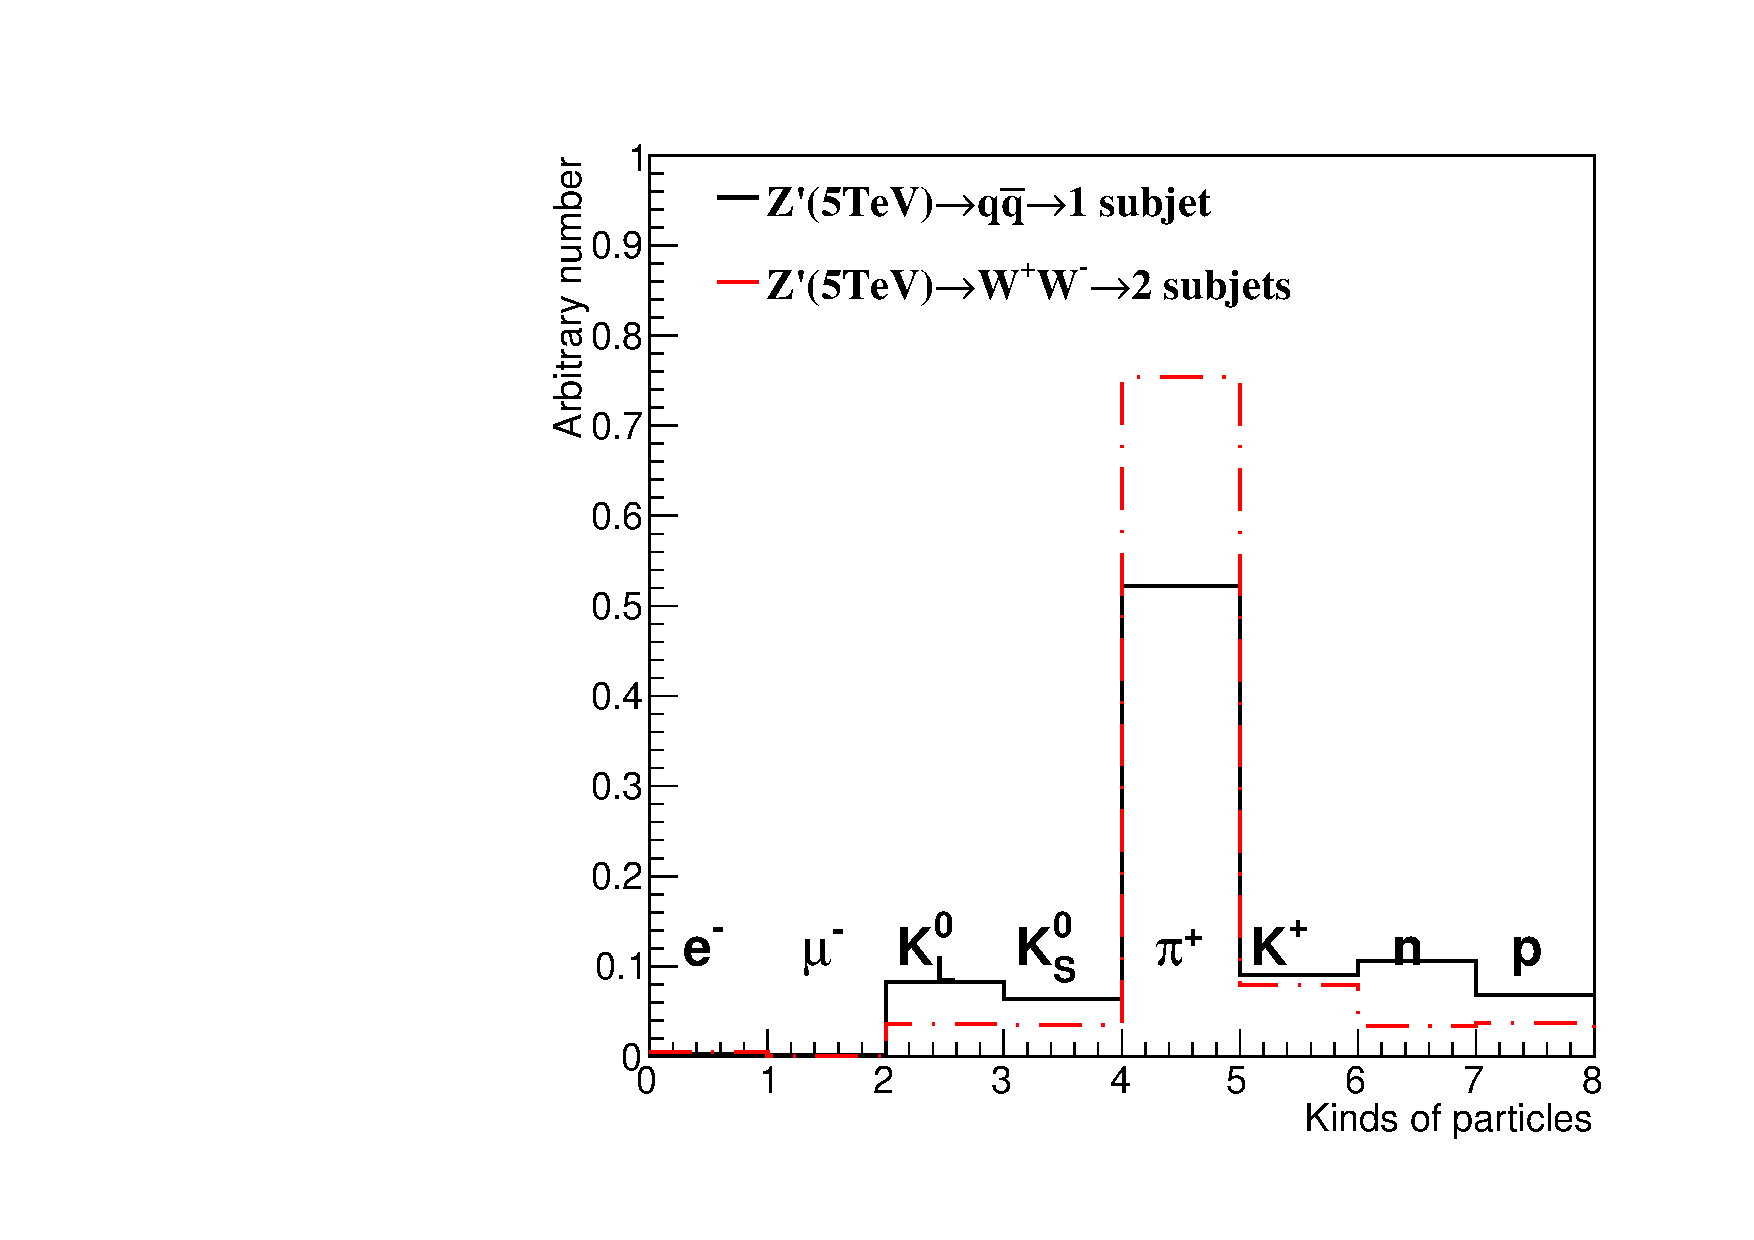
\includegraphics[width=0.45\textwidth]{/Users/ms08962476/singularity/TIming_Studies/Codes/5TeV/h_5TeV_Particles_Rank_T_0.pdf}
   }
   \subfigure[Trailing-PT] {
   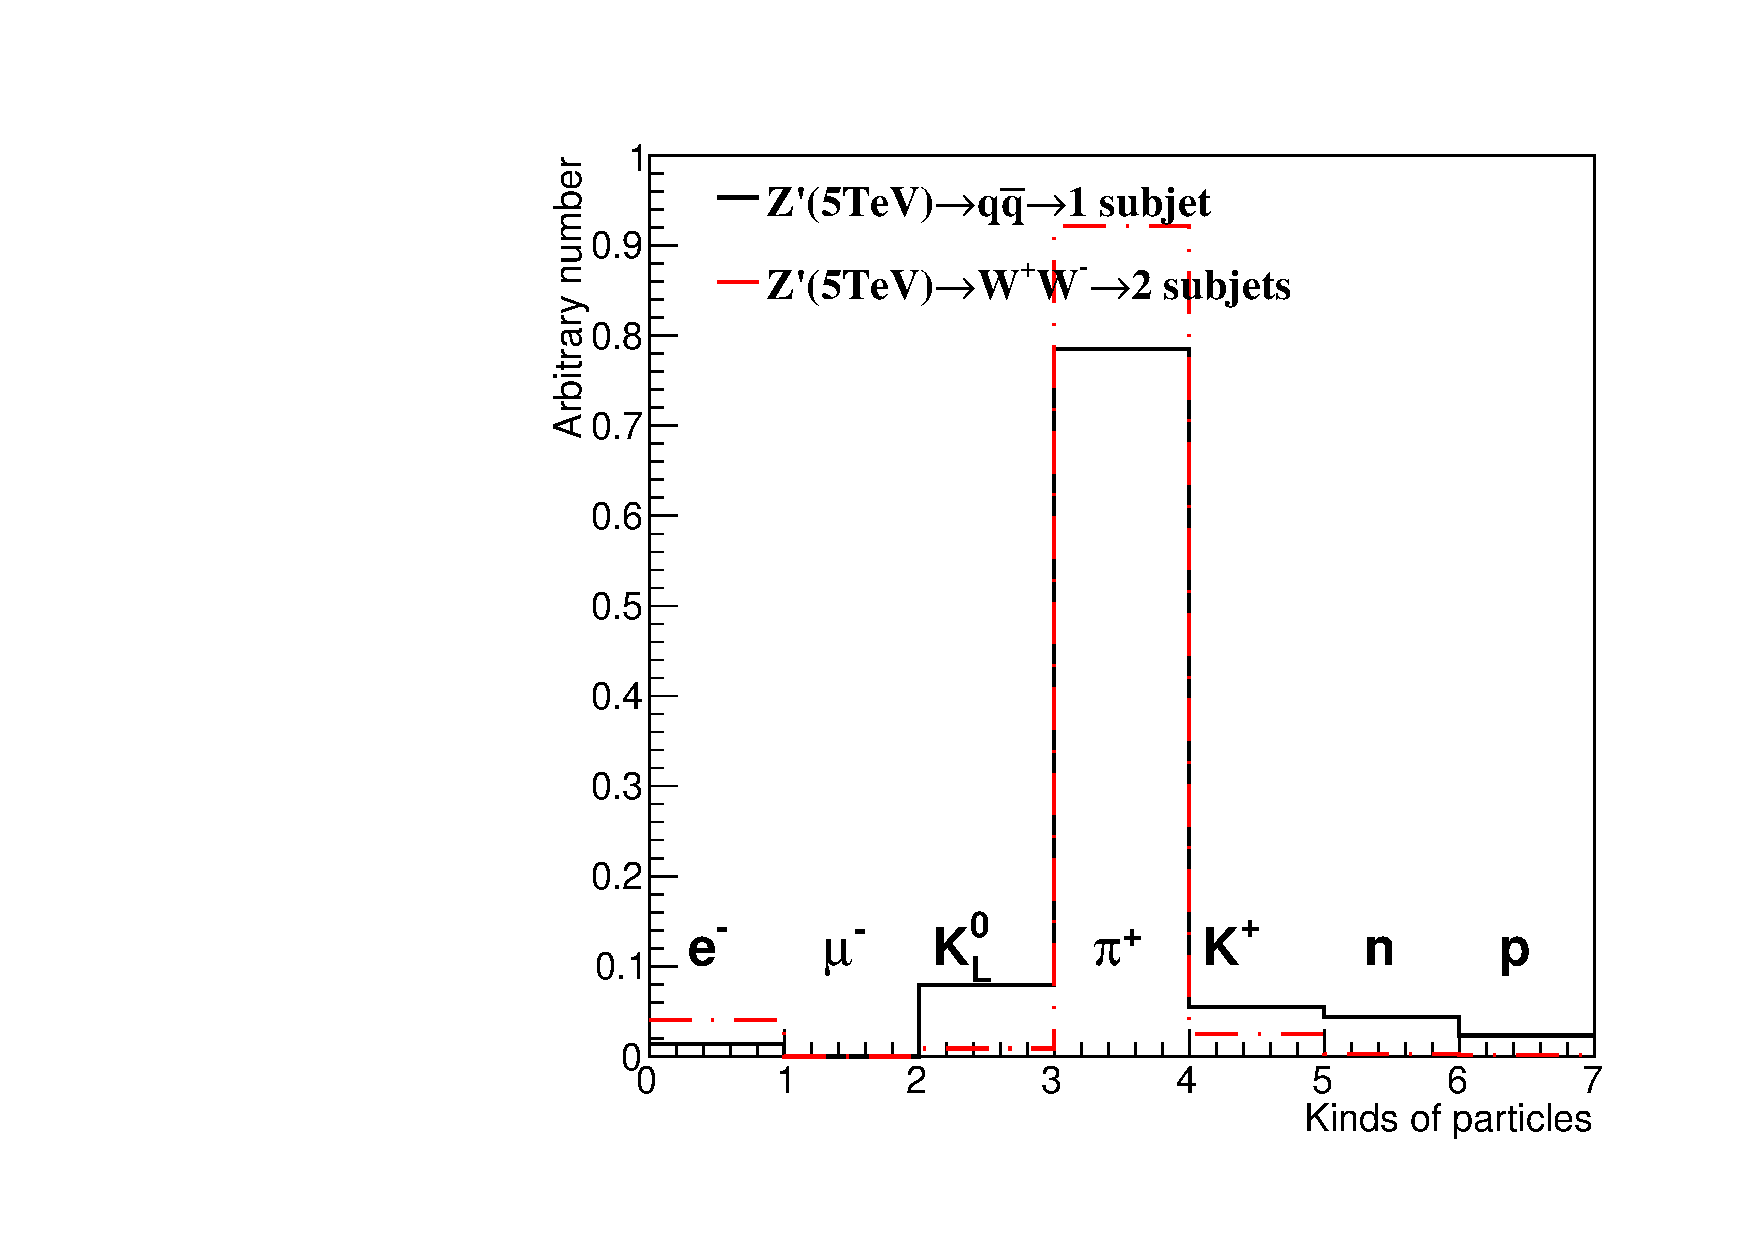
\includegraphics[width=0.45\textwidth]{/Users/ms08962476/singularity/TIming_Studies/Codes/5TeV/h_5TeV_Particles_Rank_PT_0.pdf}
   }
   \subfigure[Next-to-Trailing-T] {
   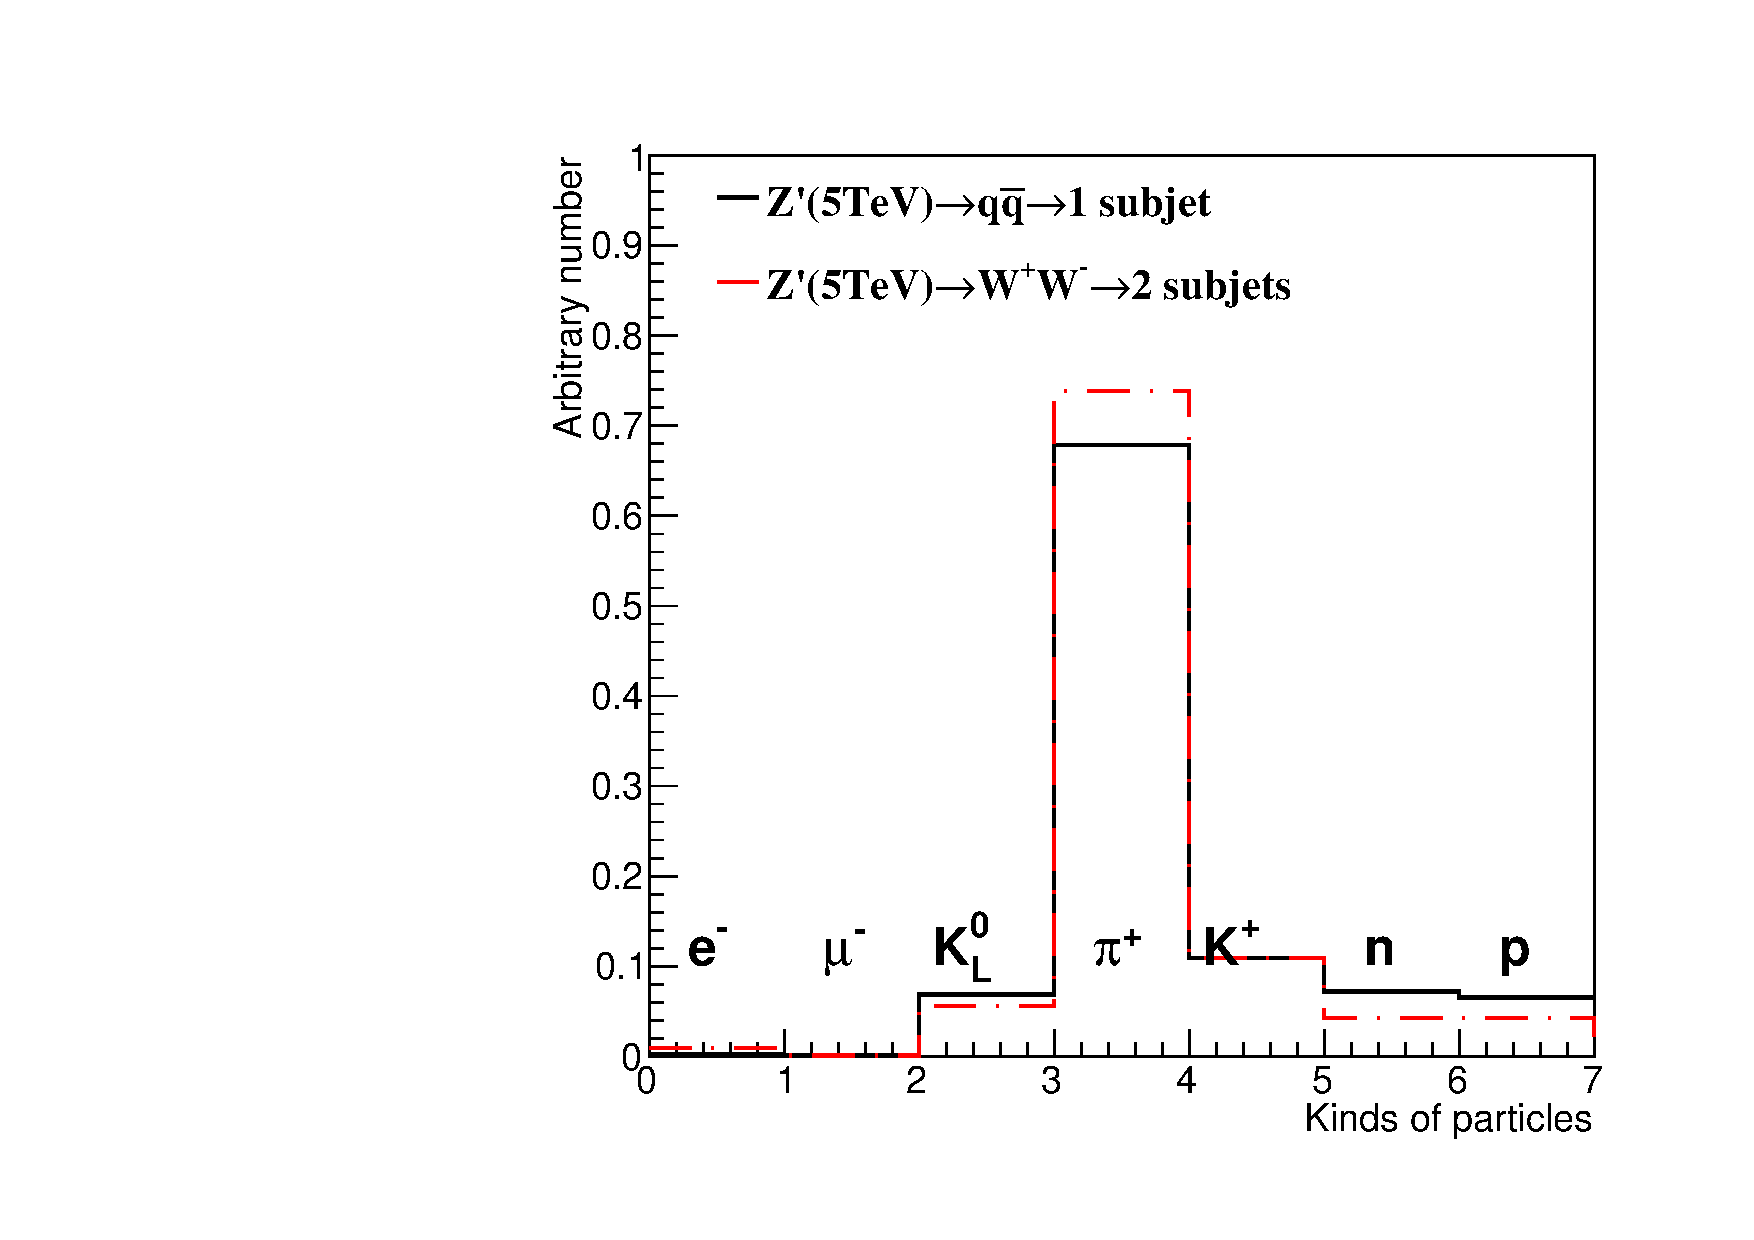
\includegraphics[width=0.45\textwidth]{/Users/ms08962476/singularity/TIming_Studies/Codes/5TeV/h_5TeV_Particles_Rank_T_1.pdf}
   }
    \subfigure[Next-to-Trailing-PT] {
   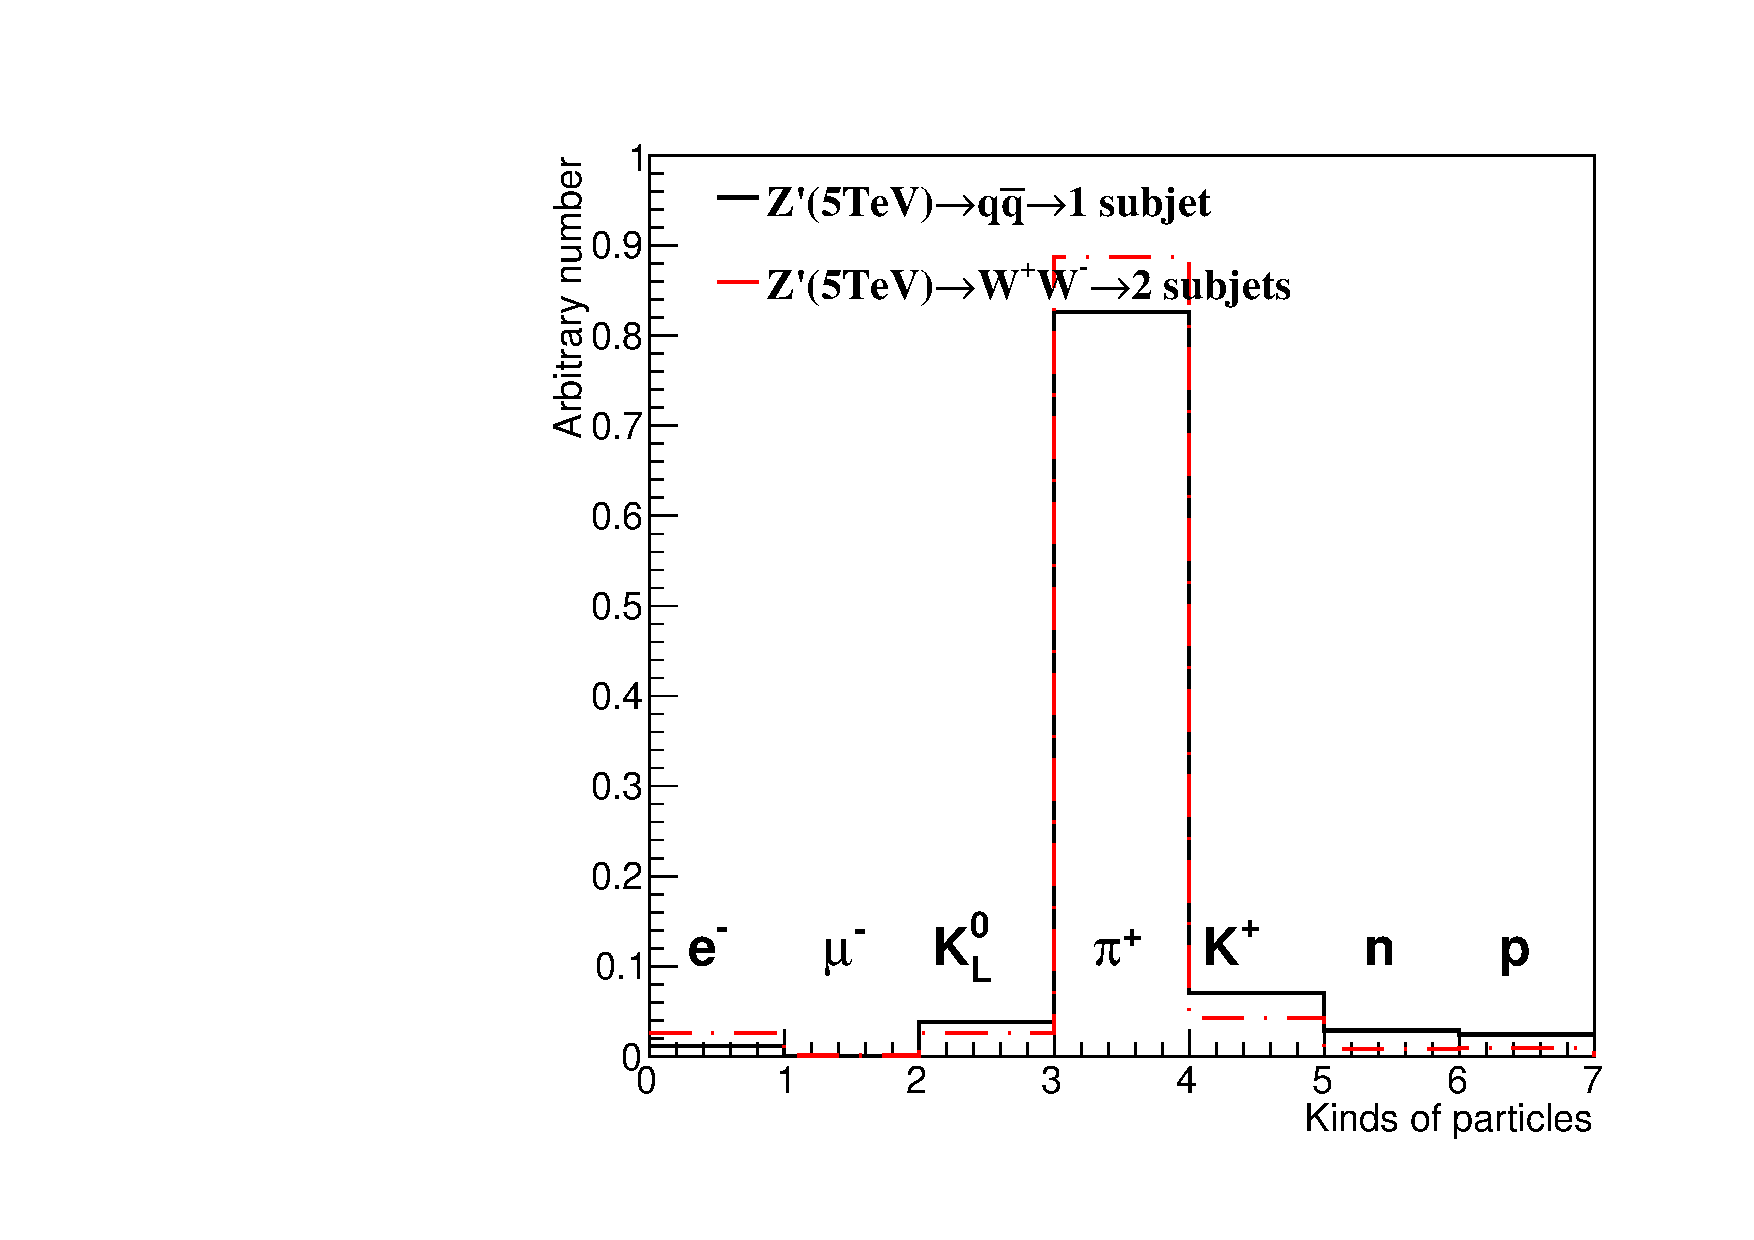
\includegraphics[width=0.45\textwidth]{/Users/ms08962476/singularity/TIming_Studies/Codes/5TeV/h_5TeV_Particles_Rank_PT_1.pdf}
   }
      \subfigure[Next-to-Next-to-Trailing-T] {
   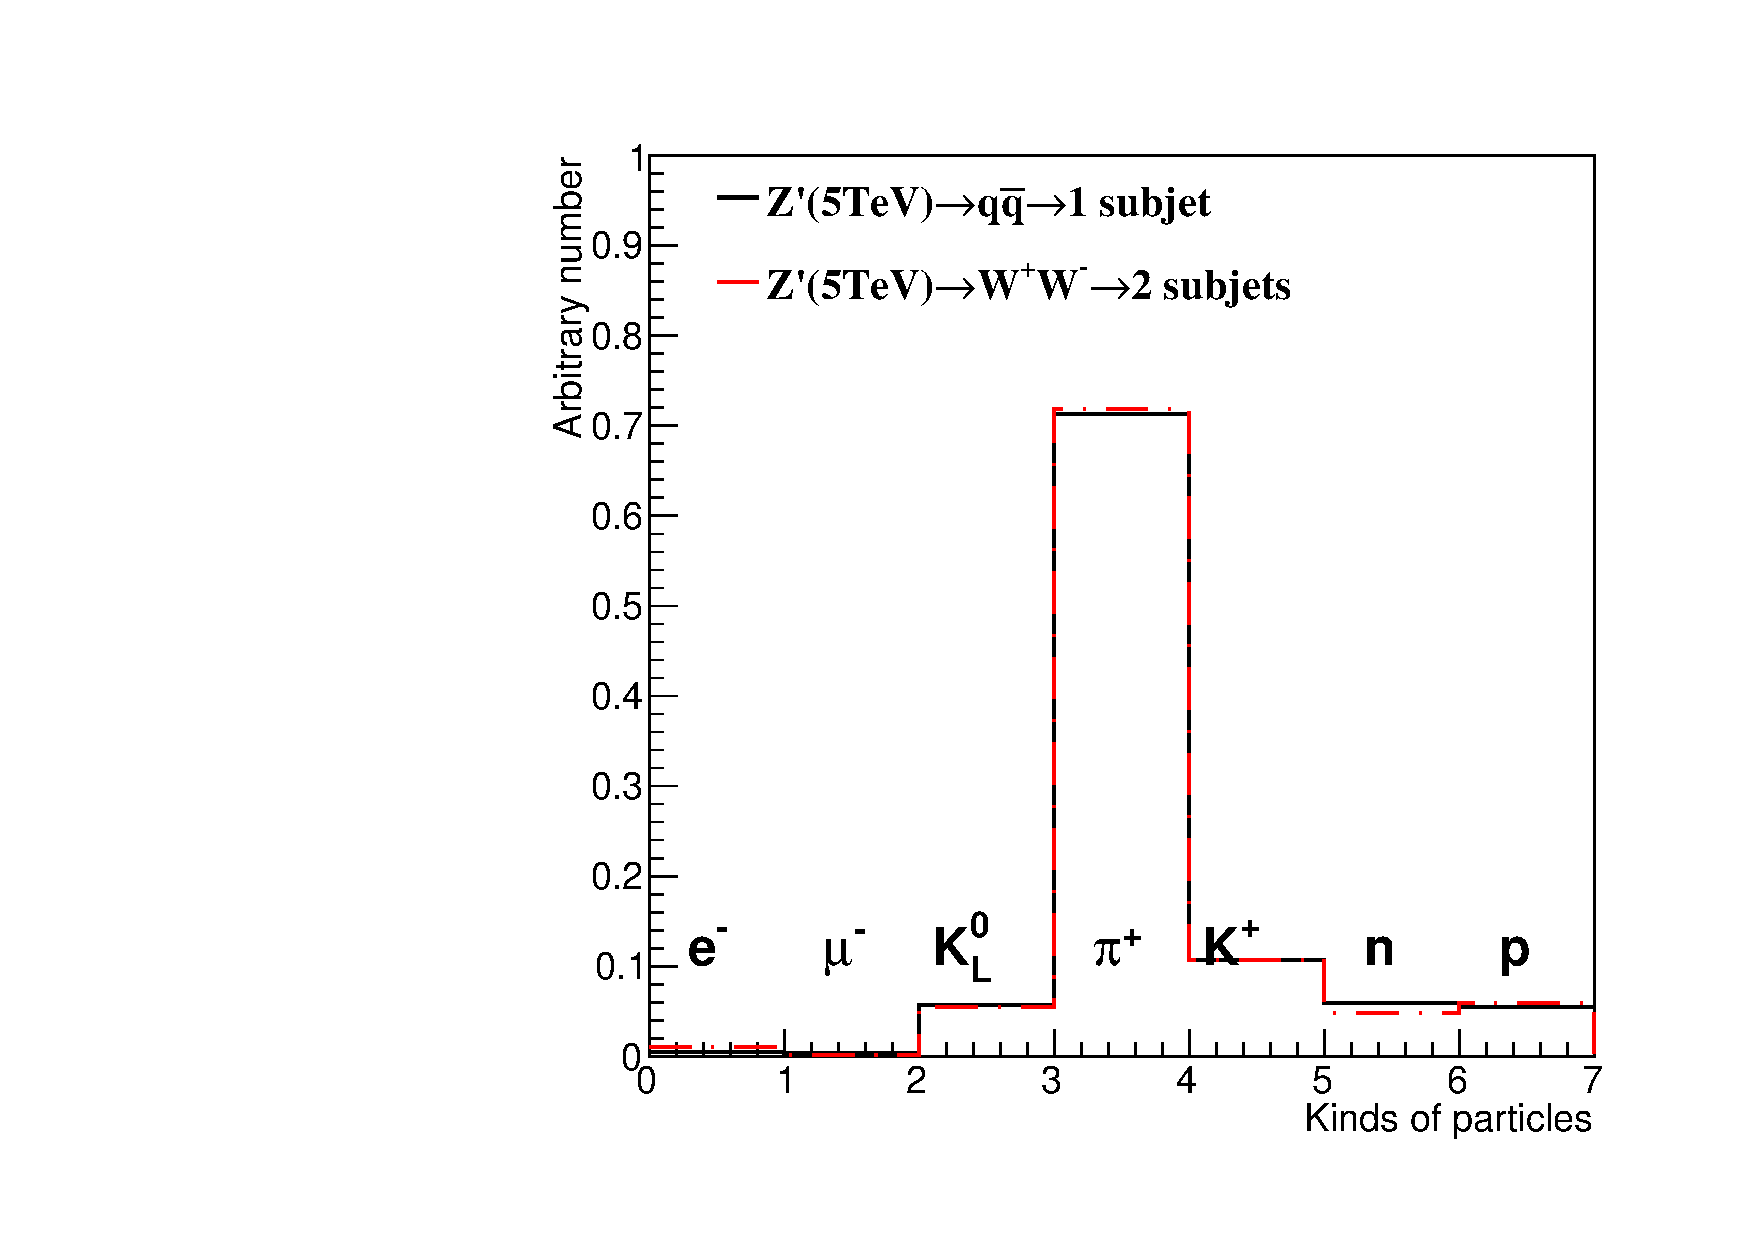
\includegraphics[width=0.45\textwidth]{/Users/ms08962476/singularity/TIming_Studies/Codes/5TeV/h_5TeV_Particles_Rank_T_2.pdf}
   }
    \subfigure[Next-to-Next-to-Trailing-PT] {
   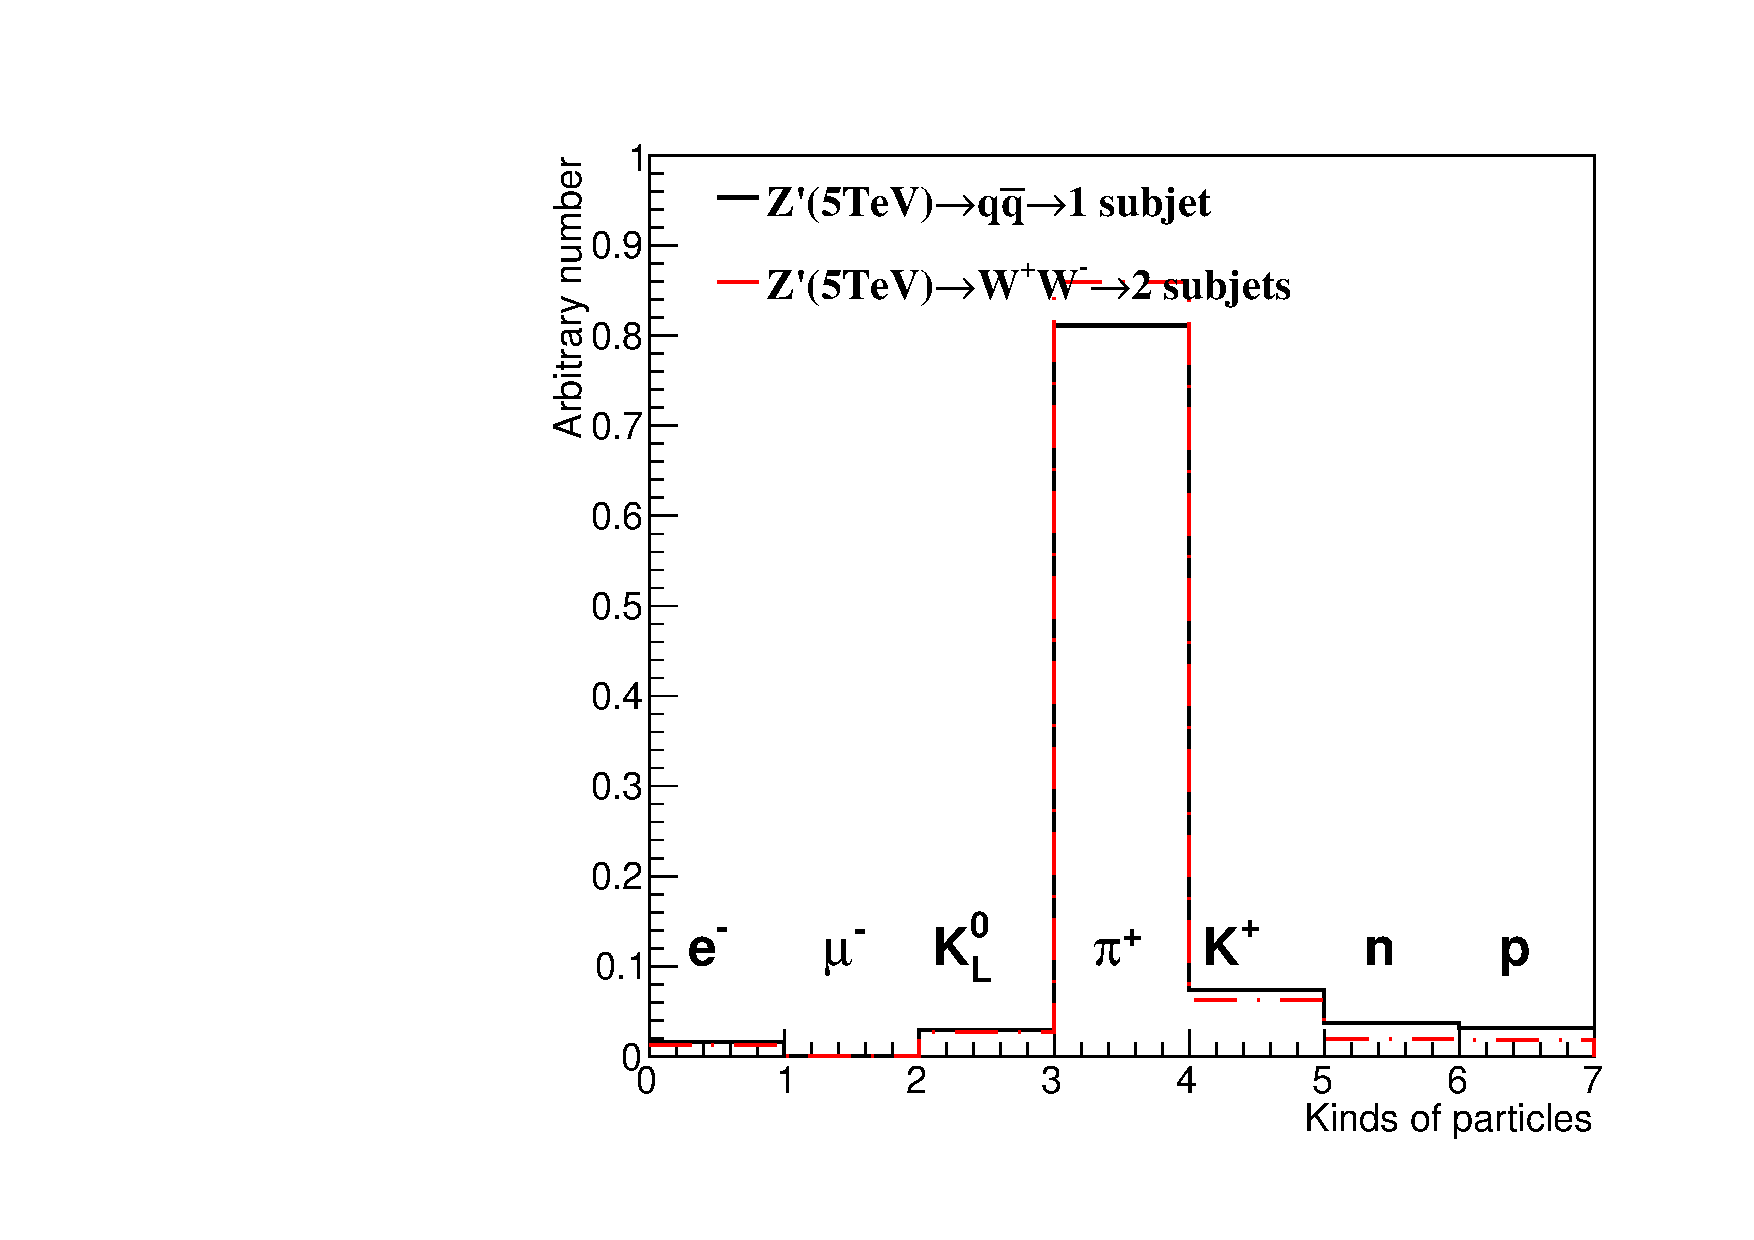
\includegraphics[width=0.45\textwidth]{/Users/ms08962476/singularity/TIming_Studies/Codes/5TeV/h_5TeV_Particles_Rank_PT_2.pdf}
   }

\end{center}
\caption{These are the particles ID of the different sorts of the trailing series with the definition of T and PT.}
\label{Particle_ID_1}
\end{figure}

\begin{figure}
\begin{center}
      \subfigure[Next-to-Next-to-Next-to-Trailing-T] {
   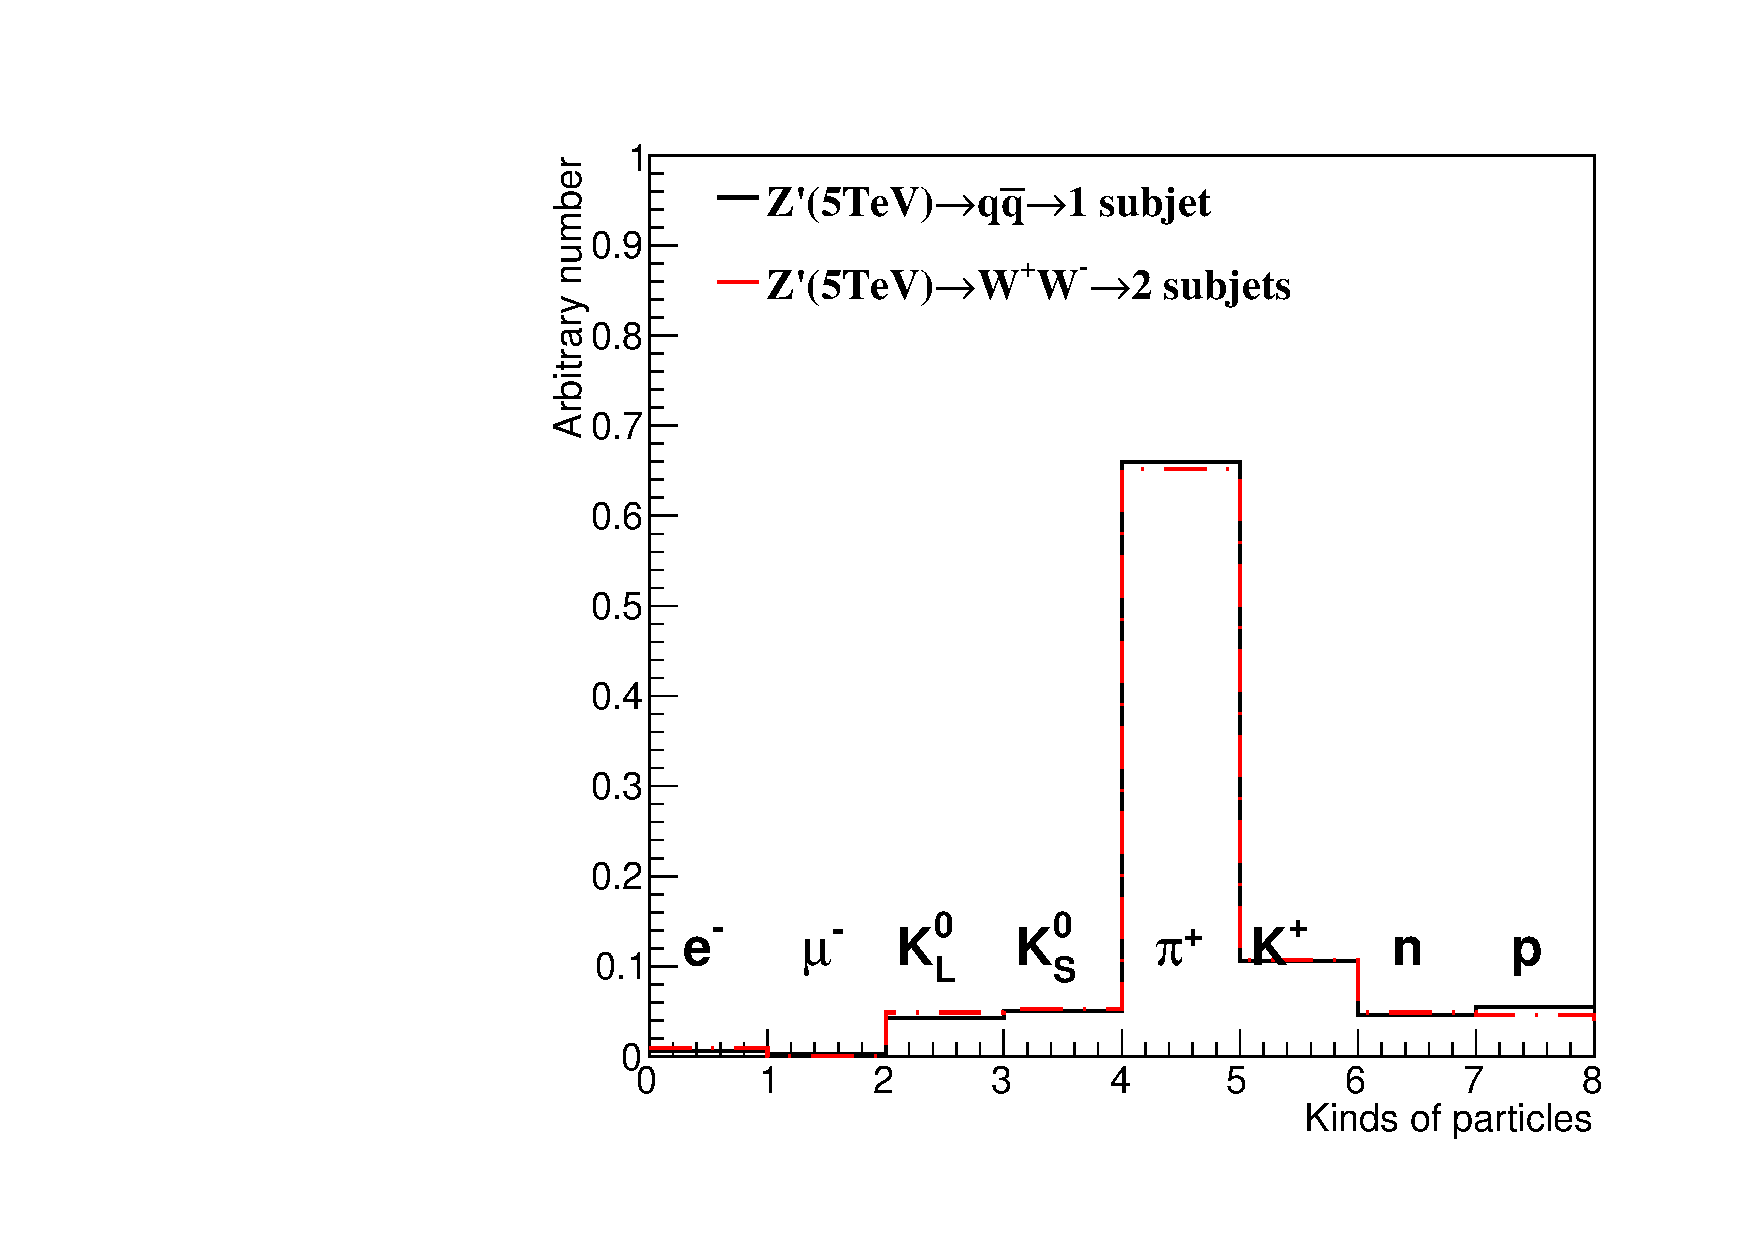
\includegraphics[width=0.45\textwidth]{/Users/ms08962476/singularity/TIming_Studies/Codes/5TeV/h_5TeV_Particles_Rank_T_3.pdf}
   }
    \subfigure[Next-to-Next-to-Next-to-Trailing-PT] {
   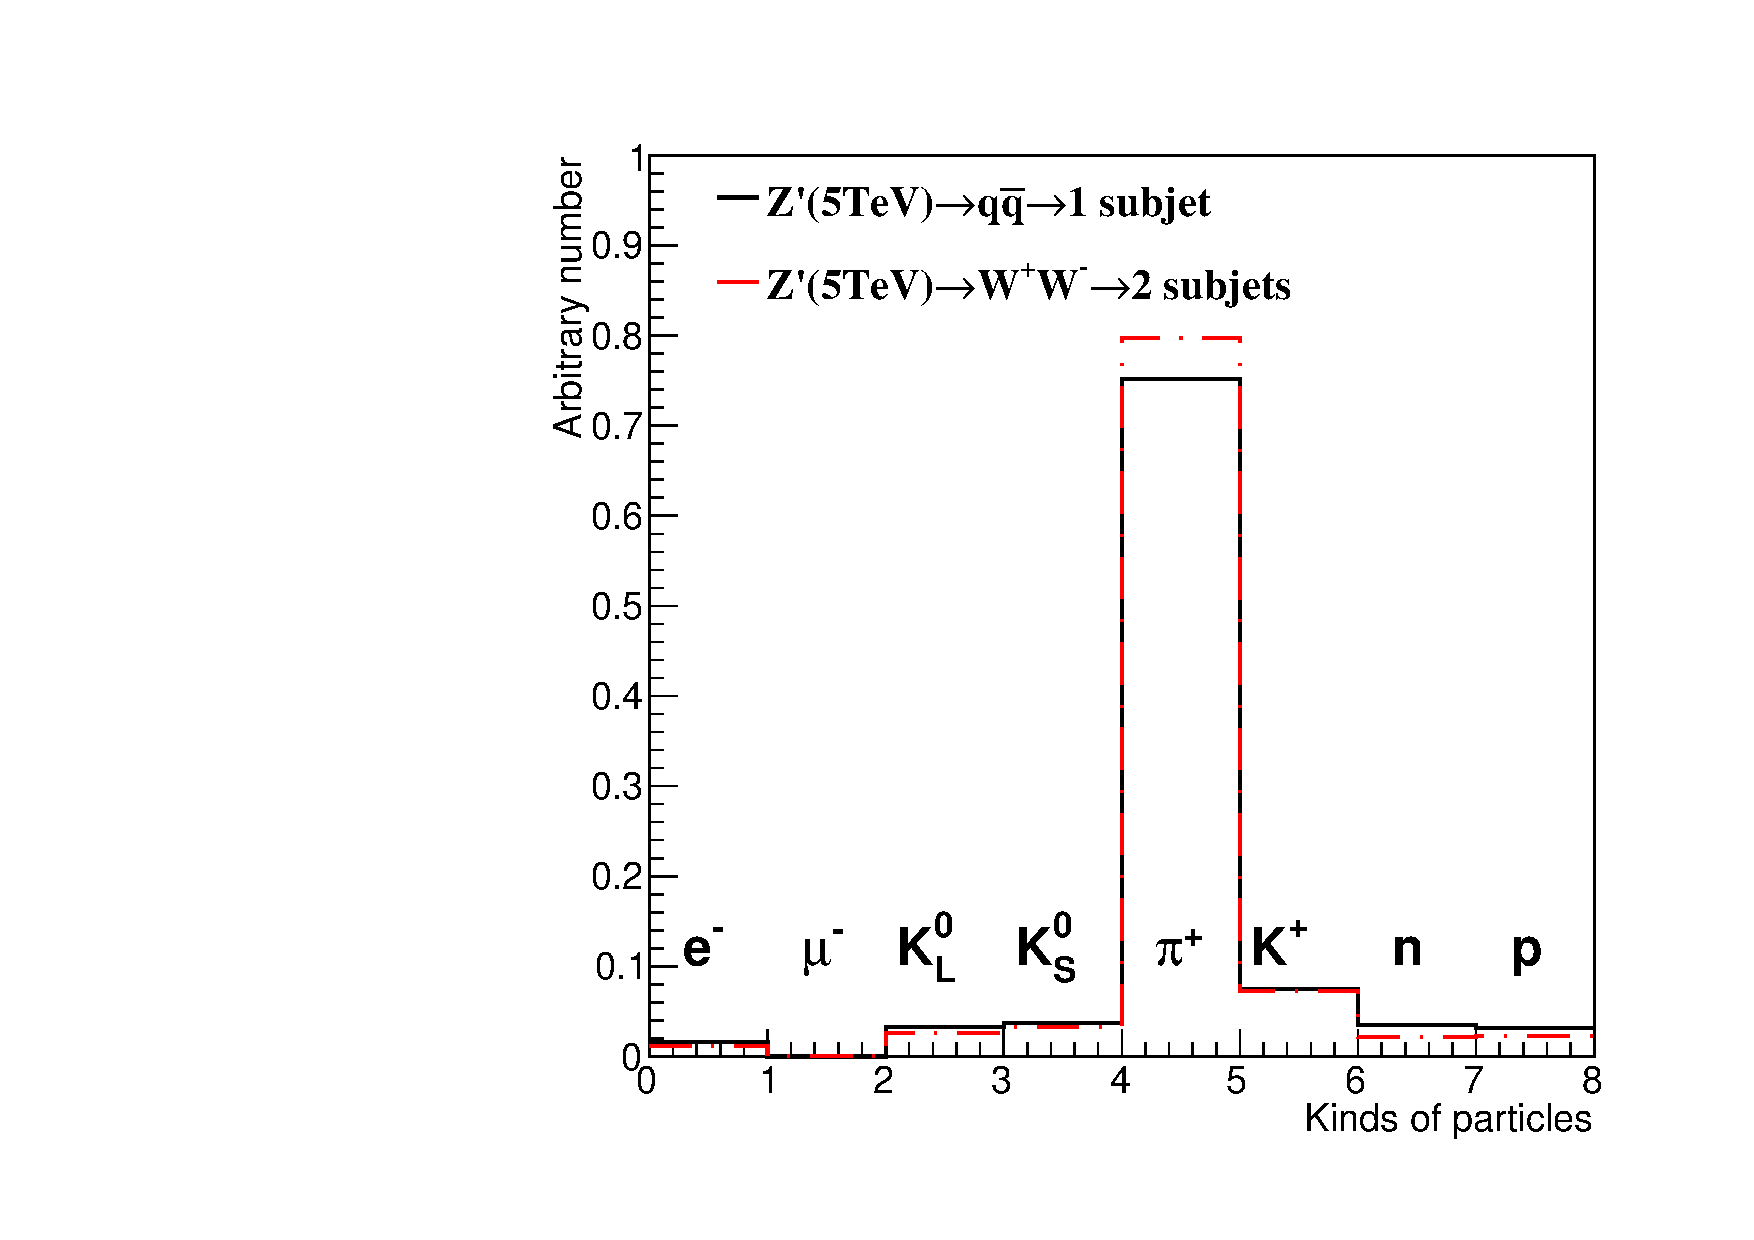
\includegraphics[width=0.45\textwidth]{/Users/ms08962476/singularity/TIming_Studies/Codes/5TeV/h_5TeV_Particles_Rank_PT_3.pdf}
   }
      \subfigure[Next-to-Next-to-Next-to-Next-to-Trailing-T] {
   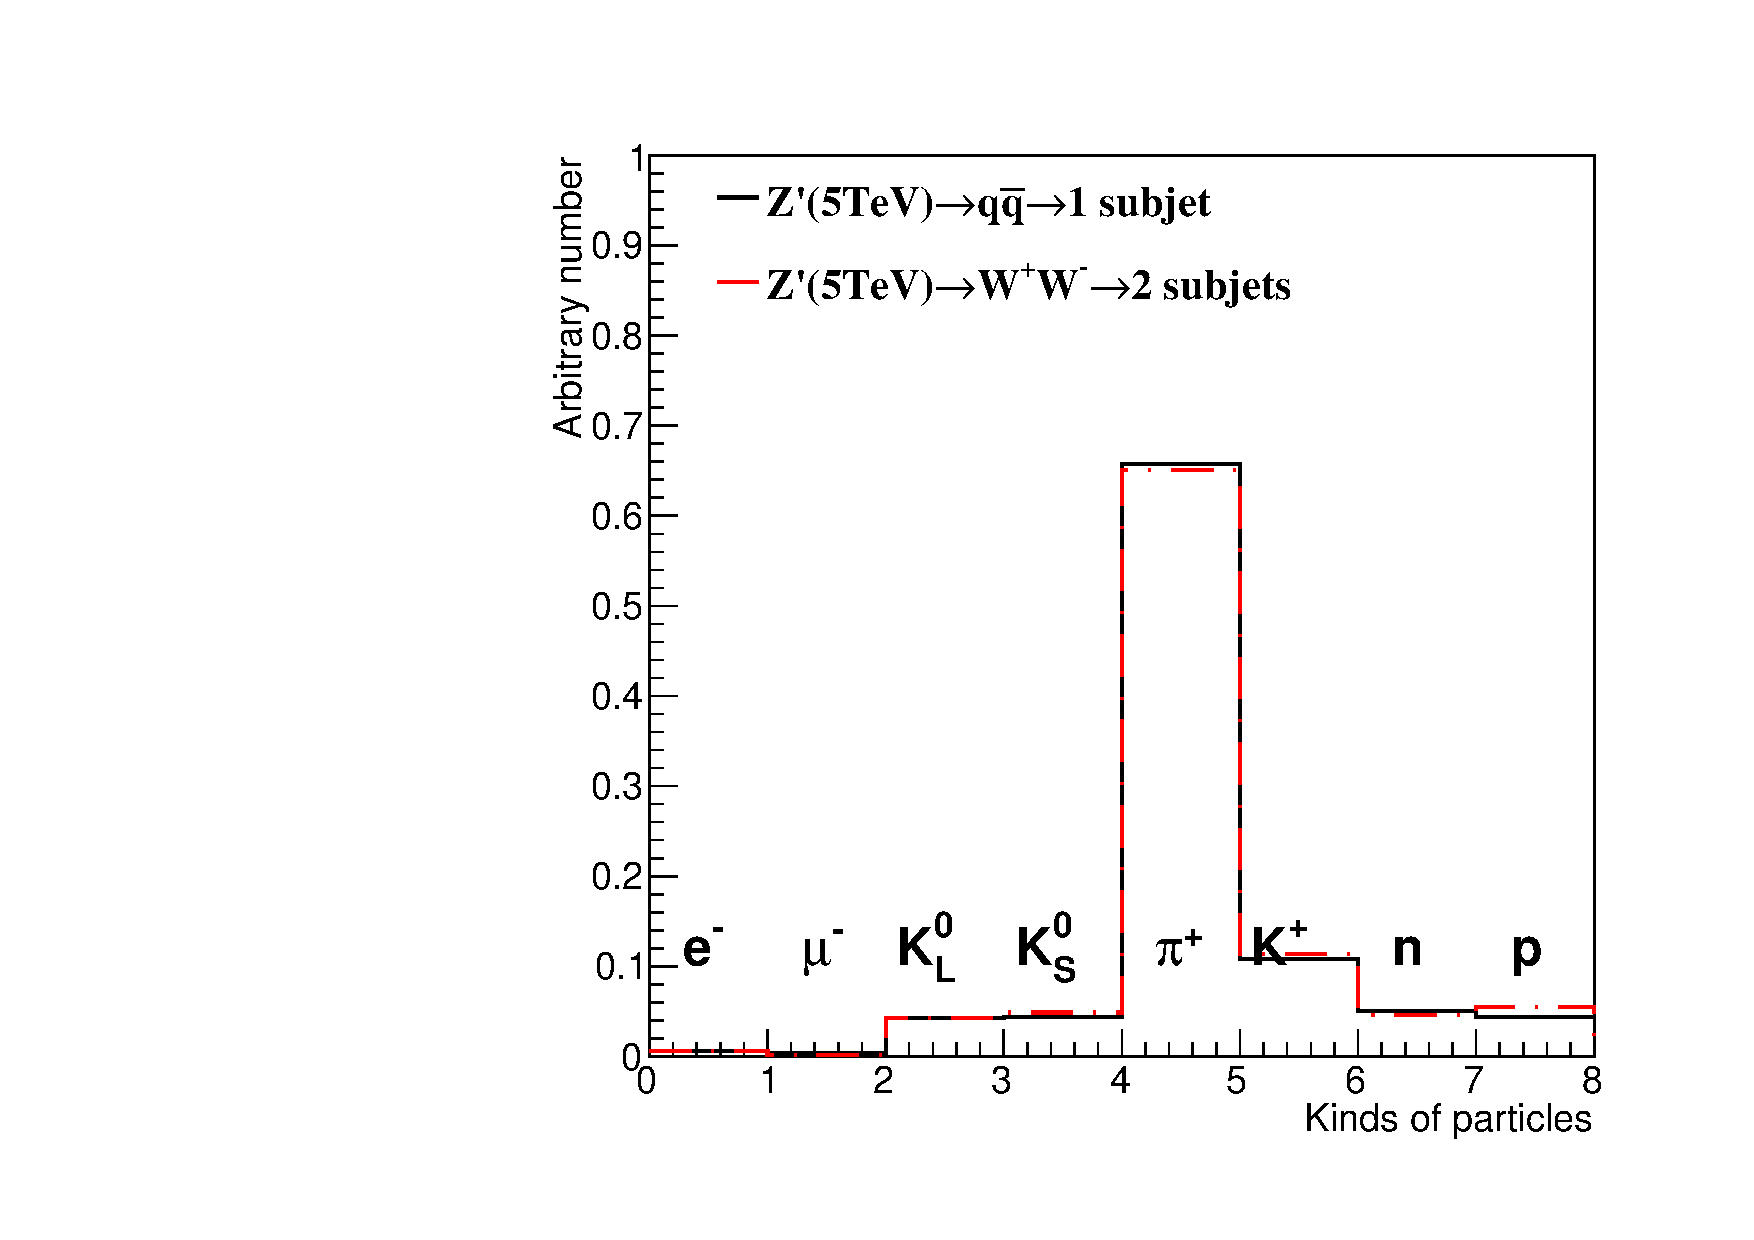
\includegraphics[width=0.45\textwidth]{/Users/ms08962476/singularity/TIming_Studies/Codes/5TeV/h_5TeV_Particles_Rank_T_4.pdf}
   }
    \subfigure[Next-to-Next-to-Next-to-Next-to-Trailing-PT] {
   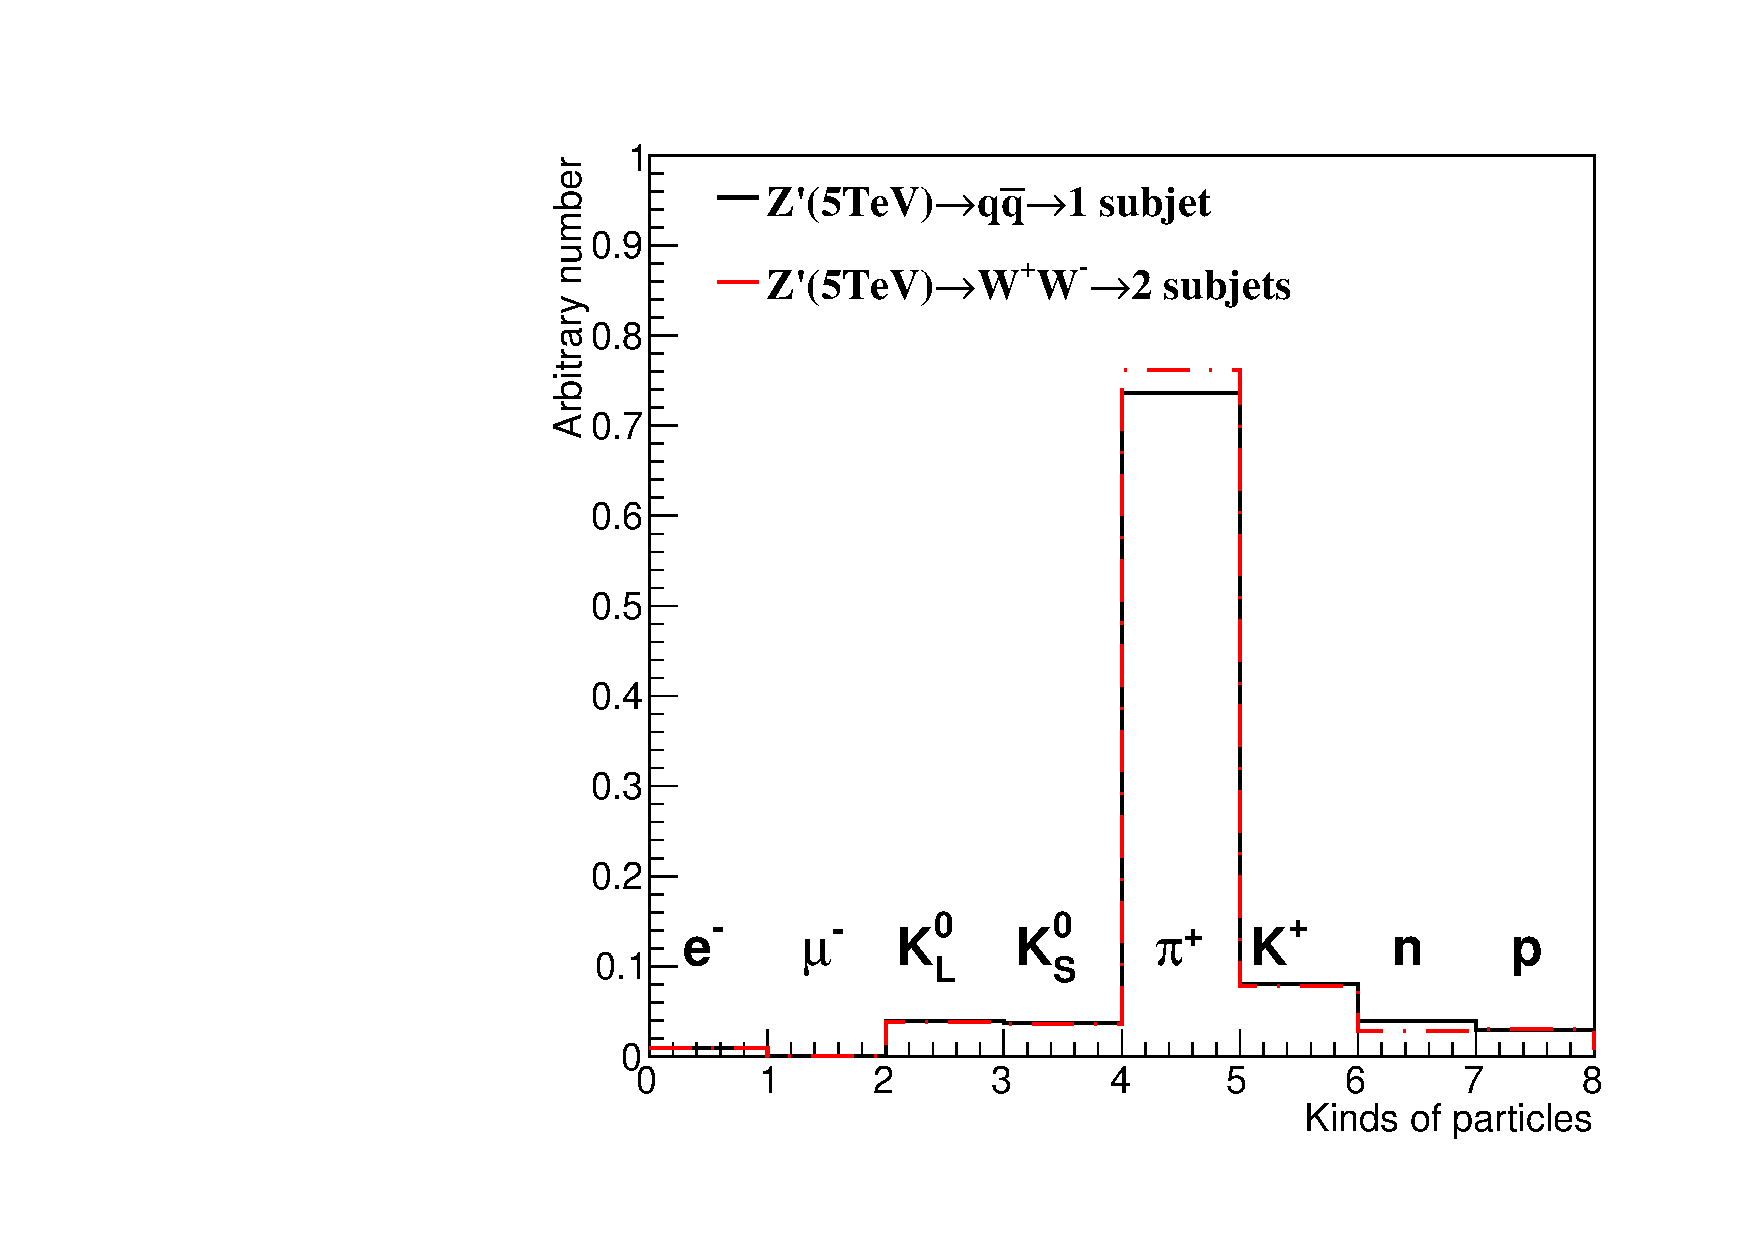
\includegraphics[width=0.45\textwidth]{/Users/ms08962476/singularity/TIming_Studies/Codes/5TeV/h_5TeV_Particles_Rank_PT_4.pdf}
   }

\end{center}
\caption{These are the particles ID of the different sorts of the trailing series with the definition of T and PT.}
\label{Particle_ID_2}
\end{figure}

%%%%%%%%%%%%%%% commented out 
\end{comment}





\newpage
%%%%%%%%%%%%%%%%%%%%%% references %%%%%%%%%%%%%%%%%%%%%%%%%%%%%%
%\section*{References}

%\bibliographystyle{elsarticle-num}
%\def\bibname{\Large\bf References}
%\def\refname{\Large\bf References}
%\pagestyle{plain}
%\bibliography{biblio}



\end{document}
